\section{Computer Vision}

\subsection{Camera Geometry (10 marks)}

$f = \SI{10}{\mm}$

$D = \SI{10}{\m} = \SI{10000}{\mm}$

$sensor: \SI{10}{\mm} \times \SI{10}{\mm} = 1000 \times 1000 \text{ pixels}$

$h = 100 \text{ pixels} = \SI{1}{\mm}$

\begin{multicols}{2}

\begin{align*}
    \frac{1}{D} + \frac{1}{d} &= \frac{1}{f} \\[1.25ex]
    \frac{1}{d} &= \frac{1}{f} - \frac{1}{D} \\[1.25ex]
    \frac{1}{d} &= \frac{1}{10} - \frac{1}{10000} \\[1.25ex]
    \frac{1}{d} &= \frac{1000}{10000} - \frac{1}{10000} \\[1.25ex]
    \frac{1}{d} &= \frac{999}{10000} \\[1.25ex]
    d &= \frac{10000}{999}
\end{align*}

\begin{align*}
    \frac{d}{D} &= \frac{h}{H} \\[1.25ex]
    H &= \frac{hD}{d} \\[1.25ex]
    H &= \frac{1 \times 10000}{\cfrac{10000}{999}} \\[1.25ex]
    H &= \SI{999}{\mm} = \SI{0.999}{\m}
\end{align*}

\end{multicols}

The observed statue is \SI{0.999}{\m} tall.

\bigskip

\begin{center}
\begin{tikzpicture}

    % horizon
    \draw[dashed] (0, 0) -- (0.82\textwidth, 0);

    % statue image
    \node[inner sep=0pt] (statue) at (1, 0.15\textwidth)
        {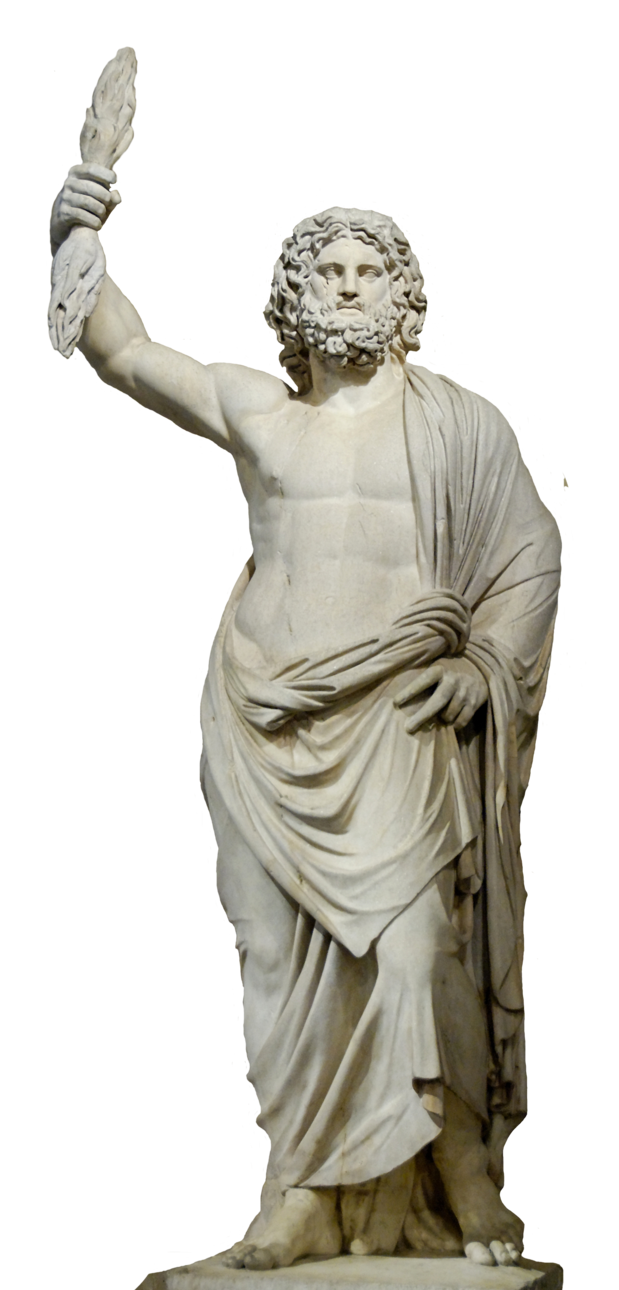
\includegraphics[height=0.3\textwidth]{res/statue.png}};

    % lens
    \draw (0.7\textwidth, 0) ellipse (1mm and 3mm);

    % film
    \draw (0.79\textwidth, -1) rectangle (0.8\textwidth, 1);

    % statue projection
    \draw (statue.north) -- (0.79\textwidth, -0.5);

    % H
    \draw[thick, <->] (statue.south west) -- (statue.north west) node[midway, anchor=east] {H};

    % D
    \draw[thick, <->] (1, -0.8) -- (0.7\textwidth, -0.8) node[midway, anchor=north] {D};

    % d
    \draw[thick, <->] (0.7\textwidth, -0.8) -- (0.79\textwidth, -0.8) node[midway, anchor=north] {d};

    % h
    \draw[thick, <->] (0.81\textwidth, 0) -- (0.81\textwidth, -0.5) node[midway, anchor=west] {h};

\end{tikzpicture}
\end{center}

\bigskip

The distance $D$ to the statue needs to be known in order to calculate the distance $d$ between the lens and the film/sensor, using the focal length $f$. Furthermore, given $D$, $d$, and $h$, it is easy to calculate the height of the statue $H$.

% - - - - - - - - - - - - - - - - - - - - - - - - - - -

\subsection{Image Processing (10 marks)}

% - - - - - - - - - - - - - - - - - - - - - - - - - - -

\subsection{Shape Recognition (10 marks)}

\newpage
